\documentclass[a4paper]{article}

  \usepackage{fullpage} % Package to use full page
  \usepackage{parskip} % Package to tweak paragraph skipping
  \usepackage{tikz} % Package for drawing
  \usepackage{tkz-graph}
  \usepackage{amsmath}
  \usepackage{siunitx} % Package for scientific units
  \usepackage{amsfonts}
  \usepackage{amssymb}
  \usepackage{hyperref}
  \usepackage[utf8]{inputenc}
  \usepackage[english]{babel}
  \usepackage{multicol}
  \usepackage{graphicx} % Package for including images
  \graphicspath{ {./images/} }
  
  \DeclareUnicodeCharacter{2212}{-}
  \newcommand\tab[1][0.5cm]{\hspace*{#1}}
  
  \title{Homework 3}
  \author{Adrian Darian}
  \date{11/5/2020}
  
  \begin{document}
  
\maketitle
  
\section*{Chapter 3}
\begin{itemize}
	\item[55] Suppose a router has built up the routing table shown in Table 3.18. The router can deliver packets directly over interfaces 0 and 1, or it can forward packets to routers R2, R3, or R4. Describe what the router does with a packet addressed to each of the following destinations:
	      \begin{itemize}
	      	\item[(a)] 128.96.39.10 \\
	      	      \textbf{Answer:} If we take the address 128.96.39.10 and apply the subnet mask rules to it we end up with the subnet number 128.96.39.0 which tells the router to send to the interface 0
	      	\item[(b)] 128.96.40.12 \\
	      	      \textbf{Answer:} If we take the address 128.96.40.12 and apply the subnet mask rules to it we end up with the subnet number 128.96.40.0 which tells the router to send to the R2
	      	\item[(c)] 128.96.40.151 \\
	      	      \textbf{Answer:} If we take the address 128.96.40.151 and apply the subnet mask rules to it we end up with the default subnet number which tells the router to send to the R4
	      	\item[(d)] 192.4.153.17 \\
	      	      \textbf{Answer:} If we take the address 192.4.153.17 and apply the subnet mask rules to it we end up with the subnet number 192.4.153.0 which tells the router to send to the R3
	      	\item[(e)] 192.4.153.90	\\
	      	      \textbf{Answer:} If we take the address 192.4.153.90 and apply the subnet mask rules to it we end up with the default subnet number which tells the router to send to the R4
	      \end{itemize} 
	      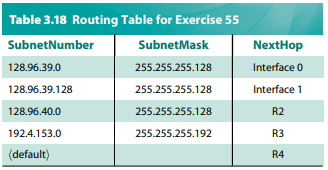
\includegraphics{3-55.png} 
	\item[58] Consider the situation involving the creation of a routing loop in the network of Figure 3.29 when the A–E link goes down. List all sequences of table updates among A, B, and C, pertaining to destination E, that lead to the loop. Assume that table updates are done one at a time, that the split-horizon technique is observed by all participants, and that A sends its initial report of E’s unreachability to B before C. You may ignore updates that don’t result in changes. \\
	      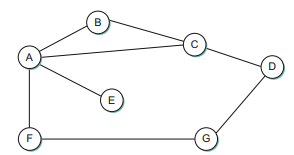
\includegraphics{3-29.png} \\
	      \textbf{Answer:} We start with the link between A and B and update saying E is unreachable. Then B links to C and tells C that E is unreach able then C links back to A and tells A that E is unreachable. This forms a loop that goes repeated until there is no longer any markers saying E is reachable.
	\item[59] Suppose a set of routers all use the split-horizon technique; we consider here under what circumstances it makes a difference if they use poison reverse in addition.
	      \begin{itemize}
	      	\item[(a)] Show that poison reverse makes no difference in the evolution of the routing loop in the two examples described in Section 3.3.2, given that the hosts involved use split horizon. \\
	      	      \textbf{Answer:} 
	      	      \begin{tabular}{c}
	      	      	$A(E, \infty)->B$ \\
	      	      	$C(E, 2)->B$      \\
	      	      	$A(E, \infty)->C$ \\
	      	      	$B(E, 3)->A$      \\
	      	      	$C(E, \infty)->B$ \\
	      	      	$A(E, 4)->C$      \\
	      	      	$B(E, \infty)->A$ \\
	      	      	$C(E, 5)->B$      \\
	      	      	$A(E, \infty)->C$ \\
	      	      	$B(E, 6)->A$      \\
	      	      \end{tabular}
	      	\item[(b)] Suppose split-horizon routers A and B somehow reach a state in which they forward traffic for a given destination X toward each other. Describe how this situation will evolve with and without the use of poison reverse. \\
	      	      \textbf{Answer:} Since we are using posion reverse A and B will follow a loop and update on the first table rather than keeping their current values and never updating.
	      	\item[(c)] Give a sequence of events that leads A and B to a looped state as in (b), even if poison reverse is used. (Hint: Suppose B and A connect through a very slow link. They each reach X through a third node, C, and simultaneously advertise their routes to each other.) \\
	      	      \textbf{Answer:} B and A send to C, C sends to A and B, finally A and B receive each other.
	      \end{itemize}	
	\item[61] Consider the network in Figure 3.58, using link-state routing. Suppose the B–F link fails, and the following then occur in sequence:
	      \begin{itemize}
	      	\item[(a)] Node H is added to the right side with a connection to G.
	      	\item[(b)] Node D is added to the left side with a connection to C.
	      	\item[(c)] A new link, D–A, is added. 
	      \end{itemize} 
	      The failed B–F link is now restored. Describe what link-state packets will flood back and forth. Assume that the initial sequence number at all nodes is 1, that no packets time out, and that both ends of a link use the same sequence number in their LSP for that link, greater than any sequence number used before. \\
	      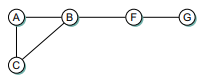
\includegraphics{3-61.png} \\
	      \textbf{Answer:} 
	      \begin{tabular}{|c|c|c|}
	      	\hline
	      	node & seq\# & connected to \\
	      	\hline
	      	A    & 2     & B, C, D      \\
	      	\hline
	      	B    & 2     & A, C         \\
	      	\hline
	      	C    & 2     & A, B, D      \\
	      	\hline
	      	D    & 2     & A, C         \\
	      	\hline
	      	F    & 2     & G            \\
	      	\hline
	      	G    & 2     & F, H         \\
	      	\hline
	      	H    & 1     & G            \\
	      	\hline
	      \end{tabular}
	\item[68] An organization has been assigned the prefix 212.1.1/24 (class C) and wants to form subnets for four departments, with hosts as follows: \\
	      \tab\tab\tab A 75 hosts \\
	      \tab\tab\tab B 35 hosts \\
	      \tab\tab\tab C 20 hosts \\
	      \tab\tab\tab D 18 hosts \\
	      There are 148 hosts in all.
	      \begin{itemize}
	      	\item[(a)] Give a possible arrangement of subnet masks to make this possible. \\
	      	      \textbf{Answer:}
	      	      \begin{tabular}{c c}
	      	      	A & 0/   \\
	      	      	B & 10/  \\
	      	      	C & 110/ \\
	      	      	D & 111/ \\
	      	      \end{tabular}
	      	\item[(b)] Suggest what the organization might do if department D grows to 32 hosts \\
	      	      \textbf{Answer:} 
	      	      \begin{tabular}{c c}
	      	      	A & 01/  \\
	      	      	  & 001/ \\
	      	      	B & 10/  \\
	      	      	C & 000/ \\
	      	      	D & 11/  \\
	      	      \end{tabular}
	      \end{itemize}
	\item[72] Table 3.20 is a routing table using CIDR. Address bytes are in hexadecimal. The notation "/12" in C4.50.0.0/12 denotes a netmask with 12 leading 1 bits: FF.F0.0.0. Note that the last three entries cover every address and thus serve in lieu of a default route. State to what next hop the following will be delivered:
	      \begin{itemize}
	      	\item[(a)] C4.5E.13.87 \\
	      	      \textbf{Answer:} B
	      	\item[(b)] C4.5E.22.09 \\
	      	      \textbf{Answer:} A
	      	\item[(c)] C3.41.80.02 \\
	      	      \textbf{Answer:} E
	      	\item[(d)] 5E.43.91.12 \\
	      	      \textbf{Answer:} F
	      	\item[(e)] C4.6D.31.2E \\
	      	      \textbf{Answer:} C
	      	\item[(f)] C4.6B.31.2E \\
	      	      \textbf{Answer:} D
	      \end{itemize}  
	      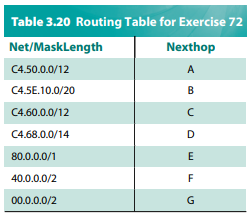
\includegraphics{3-72.png}  
\end{itemize}

\section*{Chapter 4}
\begin{itemize}
	\item[5] Suppose P, Q, and R are network service providers with respective CIDR address allocations C1.0.0.0/8, C2.0.0.0/8, and C3.0.0.0/8. Each provider’s customers initially receive address allocations that are a subset of the provider’s. \\
	      \tab P has the following customers: \\
	      \tab\tab\tab PA, with allocation C1.A3.0.0/16 \\
	      \tab\tab\tab PB, with allocation C1.B0.0.0/12. \\
	      \tab Q has the following customers: \\
	      \tab\tab\tab QA, with allocation C2.0A.10.0/20 \\
	      \tab\tab\tab QB, with allocation C2.0B.0.0/16. \\
	      Assume there are no other providers or customers.
	      \begin{itemize}
	      	\item[(a)] Give routing tables for P, Q, and R assuming each provider connects to both of the others. \\
	      	      \textbf{Answer:} \\
	      	      Routing Table for P: \\
	      	      \begin{tabular}{|c|c|}
	      	      	\hline
	      	      	address      & nextHop \\
	      	      	\hline
	      	      	C2.0.0.0/8   & Q       \\
	      	      	\hline	
	      	      	C3.0.0.0/8   & R       \\
	      	      	\hline	
	      	      	C1.A3.0.0/16 & PA      \\
	      	      	\hline	
	      	      	C1.B0.0.0/12 & PB      \\
	      	      	\hline
	      	      \end{tabular} \\
	      	      Routing Table for Q: \\
	      	      \begin{tabular}{|c|c|}
	      	      	\hline
	      	      	address       & nextHop \\
	      	      	\hline
	      	      	C1.0.0.0/8    & P       \\
	      	      	\hline	
	      	      	C3.0.0.0/8    & R       \\
	      	      	\hline	
	      	      	C2.0A.10.0/20 & QA      \\
	      	      	\hline	
	      	      	C2.0B.0.0/16  & QB      \\
	      	      	\hline
	      	      \end{tabular} \\
	      	      Routing Table for R: \\
	      	      \begin{tabular}{|c|c|}
	      	      	\hline
	      	      	address    & nextHop \\
	      	      	\hline	
	      	      	C1.0.0.0/8 & P       \\
	      	      	\hline	
	      	      	C2.0.0.0/8 & Q       \\
	      	      	\hline
	      	      \end{tabular}
	      	\item[(b)] Now assume P is connected to Q and Q is connected to R, but P and R are not directly connected. Give tables for P and R. \\
	      	      \textbf{Answer:} In the routing table for P the C3.0.0.0/8 address changes its nextHop to Q. In the routing table for R the C1.0.0.0/8 changes its nextHop to Q.
	      	\item[(c)] Suppose customer PA acquires a direct link to Q, and QA acquires a direct link to P, in addition to existing links. Give tables for P and Q, ignoring R. \\
	      	      \textbf{Answer:} \\
	      	      Routing Table for P: \\
	      	      \begin{tabular}{|c|c|}
	      	      	\hline
	      	      	address       & nextHop \\
	      	      	\hline
	      	      	C2.0.0.0/8    & Q       \\
	      	      	\hline	
	      	      	C2.0A.10.0/20 & QA      \\
	      	      	\hline	
	      	      	C1.A3.0.0/16  & PA      \\
	      	      	\hline	
	      	      	C1.B0.0.0/12  & PB      \\
	      	      	\hline
	      	      \end{tabular} \\
	      	      Routing Table for Q: \\
	      	      \begin{tabular}{|c|c|}
	      	      	\hline
	      	      	address       & nextHop \\
	      	      	\hline
	      	      	C1.0.0.0/8    & P       \\
	      	      	\hline	
	      	      	C1.A3.0.0/16  & PA      \\
	      	      	\hline	
	      	      	C2.0A.10.0/20 & QA      \\
	      	      	\hline	
	      	      	C2.0B.0.0/16  & QB      \\
	      	      	\hline
	      	      \end{tabular}
	      \end{itemize}
	\item[6] In the previous problem, assume each provider connects to both others. Suppose customer PA switches to provider Q and customer QB switches to provider R. Use the CIDR longest-match rule to give routing tables for all three providers that allow PA and QB to switch without renumbering. \\
	      \textbf{Answer:} \\
	      Routing Table for P: \\
	      \begin{tabular}{|c|c|}
	      	\hline
	      	address      & nextHop \\
	      	\hline
	      	C2.0.0.0/8   & Q       \\
	      	\hline	
	      	C3.0.0.0/8   & R       \\
	      	\hline	
	      	C1.A3.0.0/16 & Q       \\
	      	\hline	
	      	C1.B0.0.0/12 & PB      \\
	      	\hline
	      	C2.0B.0.0/16 & R       \\
	      	\hline
	      \end{tabular} \\
	      Routing Table for Q: \\
	      \begin{tabular}{|c|c|}
	      	\hline
	      	address       & nextHop \\
	      	\hline
	      	C1.0.0.0/8    & P       \\
	      	\hline	
	      	C3.0.0.0/8    & R       \\
	      	\hline	
	      	C1.A3.0.0/16  & PA      \\
	      	\hline
	      	C2.0A.10.0/20 & QA      \\
	      	\hline	
	      	C2.0B.0.0/16  & R       \\
	      	\hline
	      \end{tabular} \\
	      Routing Table for R: \\
	      \begin{tabular}{|c|c|}
	      	\hline
	      	address      & nextHop \\
	      	\hline	
	      	C1.0.0.0/8   & P       \\
	      	\hline	
	      	C2.0.0.0/8   & Q       \\
	      	\hline
	      	C1.A3.0.0/16 & Q       \\
	      	\hline
	      	C2.0B.0.0/16 & QB      \\
	      	\hline
	      \end{tabular}
\end{itemize}

\section*{Chapter 5}
\begin{itemize}
	\item[6] A sender on a TCP connection that receives a 0 advertised window periodically probes the receiver to discover when the window becomes nonzero. Why would the receiver need an extra timer if it were responsible for reporting that its advertised window had become nonzero (i.e., if the sender did not probe)? \\
	      \textbf{Answer:} 
	\item[9] You are hired to design a reliable byte-stream protocol that uses a sliding window (like TCP). This protocol will run over a 1-Gbps network. The RTT of the network is 100 ms, and the maximum segment lifetime is 30 seconds.
	      \begin{itemize}
	      	\item[(a)] How many bits would you include in the AdvertisedWindow and SequenceNum fields of your protocol header? \\
	      	      \textbf{Answer:} 32 bits \\
	      	      \begin{tabular}{rcl}
	      	      	$RTT \times bandwidth$ & $=$ &              \\
	      	      	$100ms \times 1Gbps$   & $=$ & $12.5MB$     \\
	      	      	$2^24$                 & $=$ & $16 million$ \\
	      	      	$@30s$                 & $=$ & $3.75GB$     \\
	      	      	$2^32$                 & $=$ & $4GB$        
	      	      \end{tabular}
	      	\item[(b)] How would you determine the numbers given above, and which values might be less certain? \\
	      	      \textbf{Answer:} RTT and bandwidth are mesaurements from the hardware/software.
	      \end{itemize}
	\item[12] Suppose TCP operates over a 1-Gbps link.
	      \begin{itemize}
	      	\item[(a)] Assuming TCP could utilize the full bandwidth continuously, how long would it take the sequence numbers to wrap around completely? \\
	      	      \textbf{Answer:} $\frac{2^32}{125MB/sec} = 32 seconds$
	      	\item[(b)] Suppose an added 32-bit timestamp field increments 1000 times during the wraparound time you found above. How long would it take for the timestamp to wrap around? \\
	      	      \textbf{Answer:} $32 bit \times 4 \times 10^9 ms = 128000000s$
	      \end{itemize}
	\item[14] If host A receives two SYN packets from the same port from remote host B, the second may be either a retransmission of the original or, if B has crashed and rebooted, an entirely new connection request.
	      \begin{itemize}
	      	\item[(a)] Describe the difference as seen by host A between these two cases. \\
	      	      \textbf{Answer:} the packets ID will be the same if they are duplicates
	      	\item[(b)] Give an algorithmic description of what the TCP layer needs to do upon receiving a SYN packet. Consider the duplicate/ new cases above and the possibility that nothing is listening to the destination port. \\
					\textbf{Answer:} \\
					if (Transport.accept(layerPort)) Sender.send(RST) \\
					else if (!Transport.contains($T<layerPort, receiveraddr, receiverPort>$)) \\
					\tab Transport.insert($T,<layerPort, receiveraddr, receiverPort>$) \\
					\tab Transport.set(receiverID) \\
					\tab Transport.set(layerId) \\
					\tab Sender.send(SYN\_ACK) \\
					\tab socket.state = SYN\_RCVD \\
					else if (Transport.contains($T<layerPort, receiveraddr, receiverPort>$)) \\
					\tab if (receiverId == layerID) // duplicate \\
					\tab else Sender.send(RST)
	      \end{itemize}
	\item[19] If a packet arrives at host A with B’s source address, it could just as easily have been forged by any third host C. If, however, A accepts a TCP connection from B, then during the three-way handshake A sent ISNA to B’s address and received an acknowledgment of it. If C is not located so as to be able to eavesdrop on ISNA, then it might seem that C could not have forged B’s response. However, the algorithm for choosing ISNA does give other unrelated hosts a fair chance of guessing it. Specifically, A selects ISNA based on a clock value at the time of connection. Request for Comments 793 specifies that this clock value be incremented every $\SI{4}{\mu}s$; common Berkeley implementations once simplified this to incrementing by 250,000 (or 256,000) once per second.
	      \begin{itemize}
	      	\item[(a)] Given this simplified increment-once-per-second implementation, explain how an arbitrary host C could masquerade as B in at least the opening of a TCP connection. You may assume that B does not respond to SYN + ACK packets A is tricked into sending to it. \\
	      	      \textbf{Answer:} First step is where C establishes a connection to A so that is may have access to read A's clock ID. Then C will begin sending packets to A as SYN packets. While A sends similar packets to B but as SYN\_ACK packets. C then sends the appropriate ACK packet to A along with a payload of data that will be read at B. Finally the established connection will remain open or reset.
	      	\item[(b)] Assuming real RTTs can be estimated to within 40 ms, about how many tries would you expect it to take to implement the strategy of part (a) with the unsimplified "increment every $\SI{4}{\mu}s$" TCP implementation? \\
	      	      \textbf{Answer:} $\frac{40ms}{\SI{4}{\mu}sec} = 10,000$
	      \end{itemize} 
\end{itemize}

\section*{Extra Credit:}

In the language of your choice, write a program that opens up a TCP connection to the machine www.andes.ucmerced.edu on port 80. Your program should send the following string: \\
$GET / HTTP/1.1\backslash r\backslash n\backslash r\backslash n$ \\
(Where $\backslash r$ and $\backslash n$ are the ASCII characters 0xd0 and 0xa0, respectively.) \\
Then your program should read data that is sent back to you on that same TCP connection, and print it out. \\
Email us a .tar.gz file with your source code, and instructions on<br>how to compile and run it.

\end{document}